\documentclass[12pt,a4paper]{article}
\usepackage[utf8]{inputenc}
\usepackage[german]{babel}
\usepackage[T1]{fontenc}
\usepackage{amsmath}
\usepackage{amsfonts}
\usepackage{amssymb}
\usepackage{graphicx}
\usepackage[left=2.5cm,right=2.5cm,top=2cm,bottom=2cm]{geometry}
\usepackage{float}
\author{Gruppe C14 \\ Julián Häck, Martin Koytek, Lars Wenning, Erik Zimmermann}
\begin{document}
\section{Bestimmung der Schallgeschwindigkeit durch Laufzeitmessung}
\subsection{Versuchsbeschreibung}
%Kurze Darstellung der physikalischen Grundlagen und Ziele der Versuche, %die zum Verständnis
%des Versuches/Protokolls benötigt werden. (max. 1 Seite)
Bei der Bestimmung der Schallgeschwindigkeit in Luft durch eine Laufzeitmessung wird eine Störung in verschiedenen Abständen aufgezeichnet, um anschließend den Abstand gegen die vom Schall benötigte Zeit zum Zurücklegen dieser Strecke aufgetragen. Aus der Steigung der durch die Messwerte gefitteten Geraden ergibt sich somit die Schallgeschwindigkeit:
\begin{equation}
v=\frac{s}{t}
\end{equation}
Für die Temperaturabhängigkeit gilt:
\begin{equation}
v=v_0\cdot \sqrt{\frac{T}{T_0}} \label{Temperaturabhängigkeit}
\end{equation} 
\subsection{Versuchsaufbau und Durchführung}
%Genaue Beschreibung der verwendeten Aufbauten unter Verwendung von Skizzen oder Photos
%Beschreibung der Messwerterfassungseinstellungen (eingestellte Messzeiten, Messbedingungen,
%Trigger, Anzahl der Messungen) und der Durchführung der Versuche. (max. 1 Seite)
\begin{figure}[H]
\centering
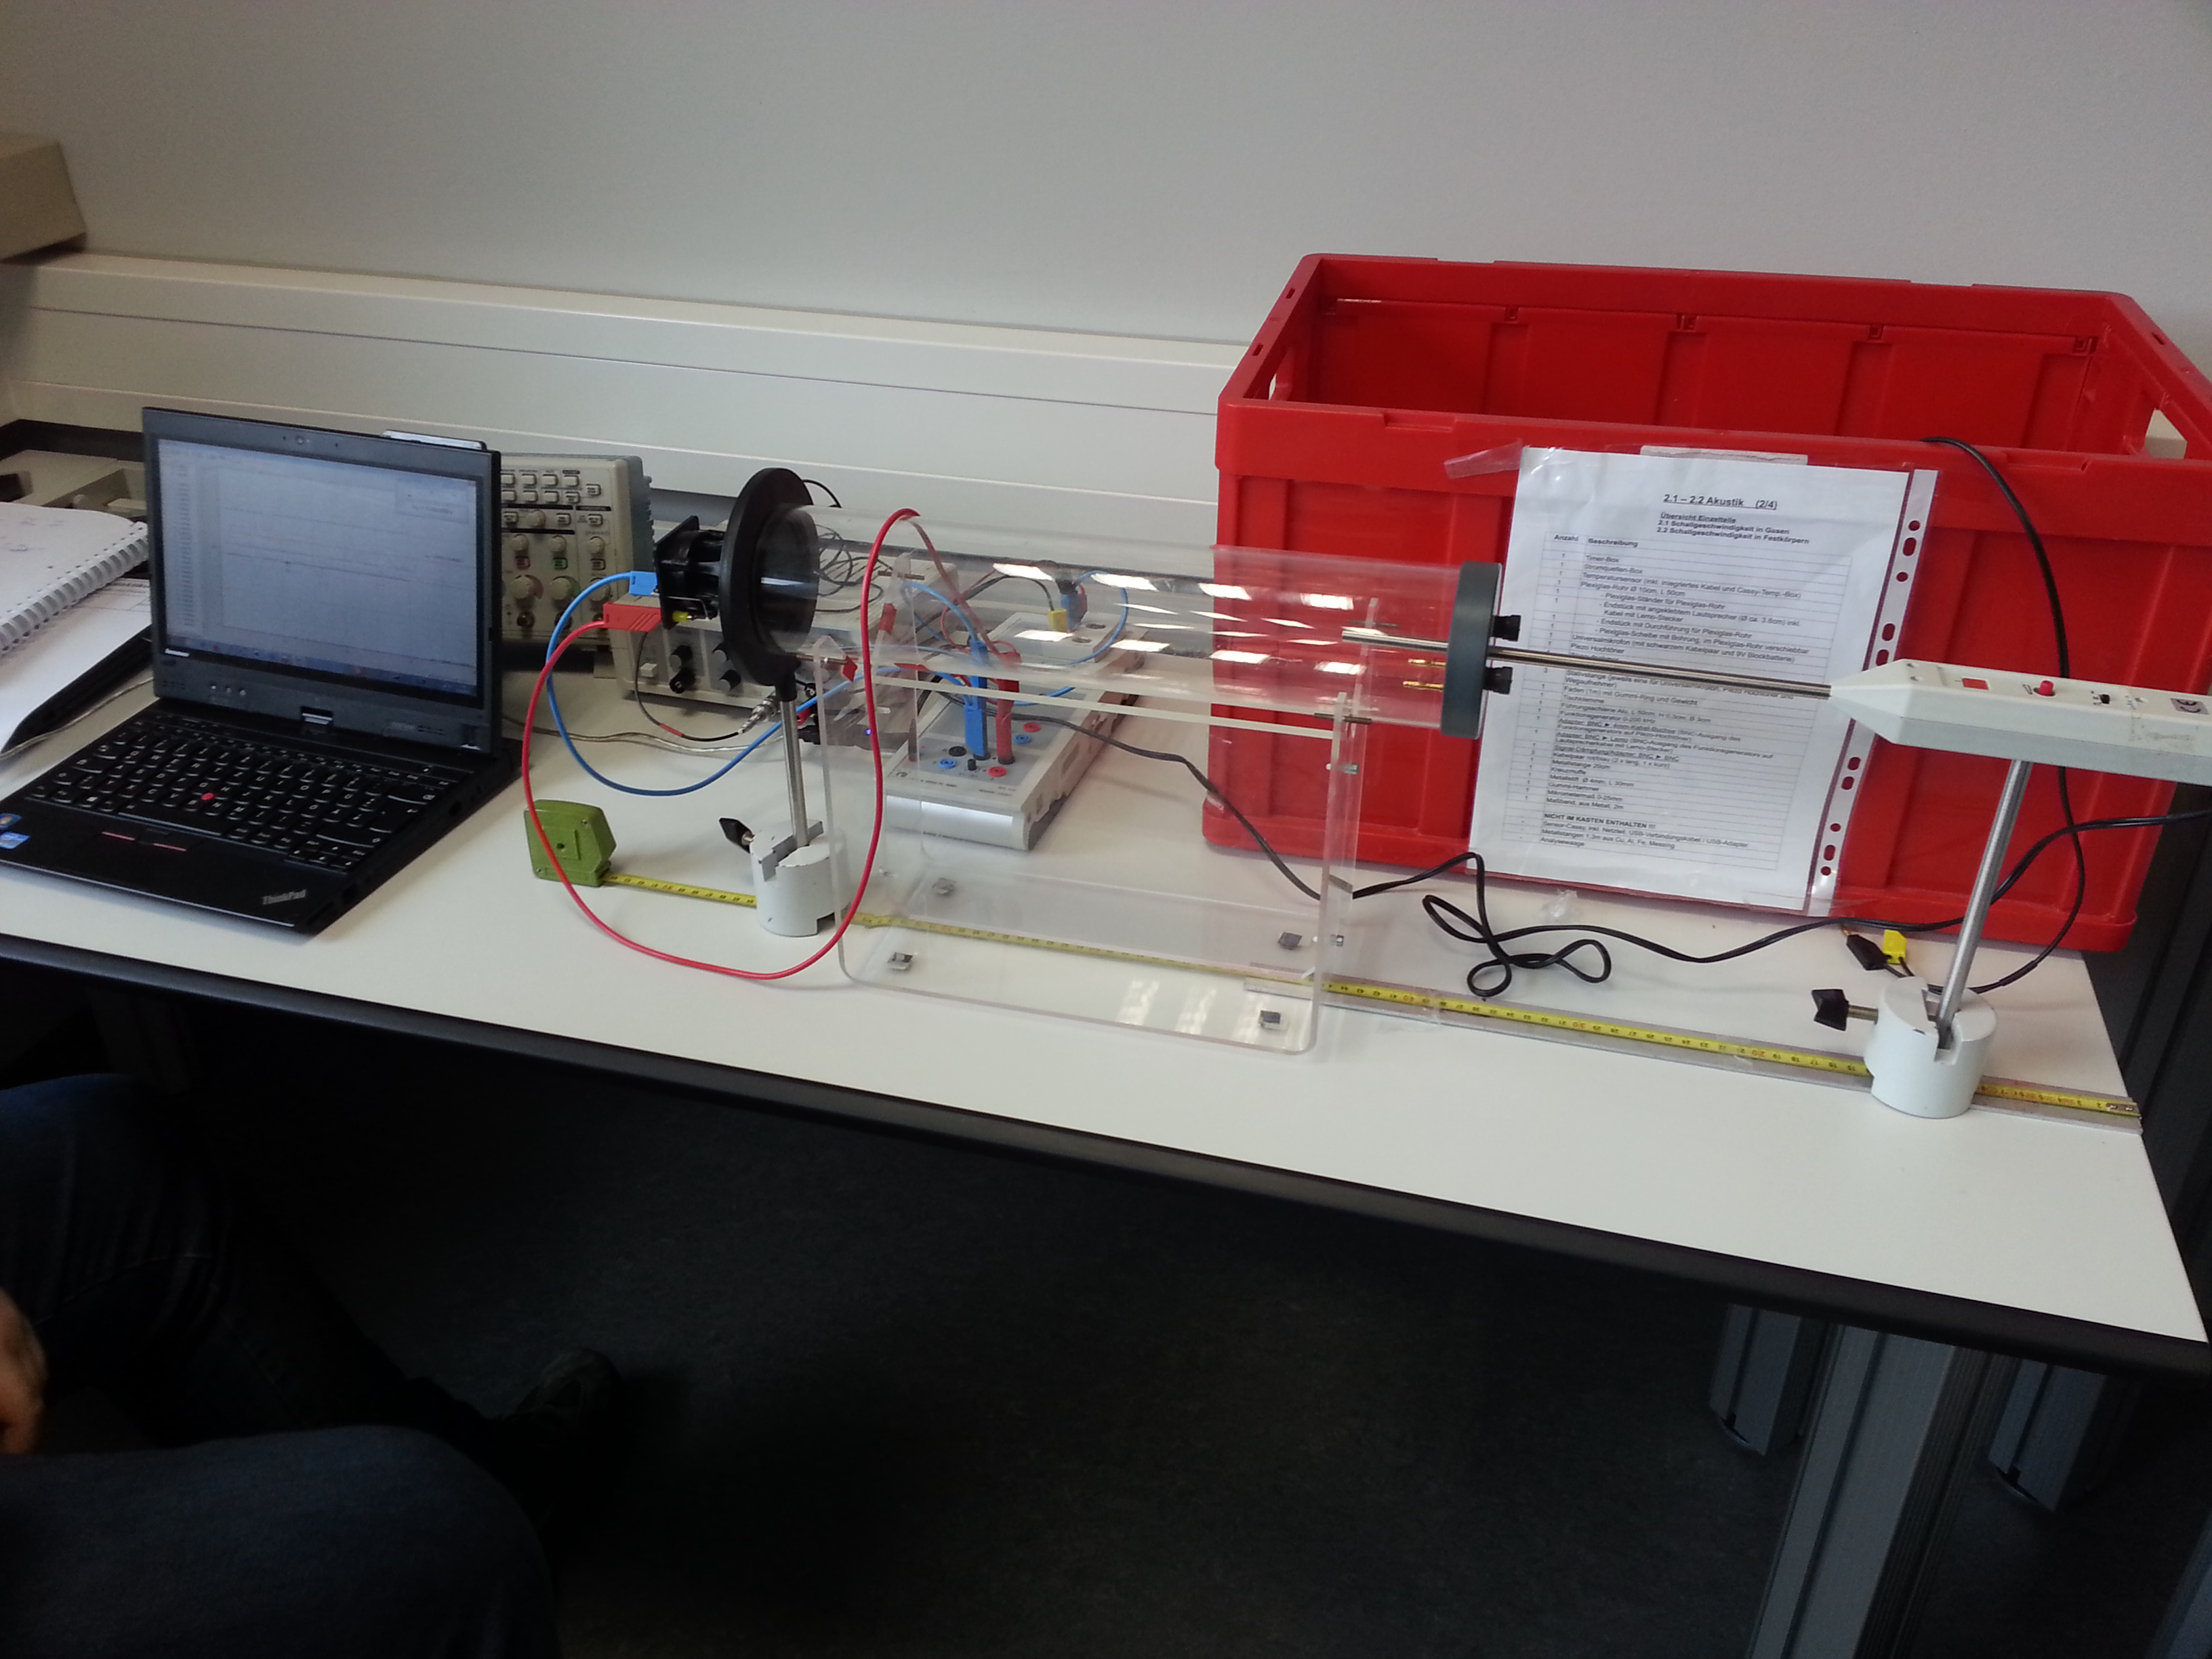
\includegraphics[scale=0.15]{Bilder/laufzeit-cassy.jpg}
\caption{Versuchsaufbau der Laufzeitmessung mit dem Sensor-Cassy.}
\end{figure}
\begin{figure}[H]
\centering
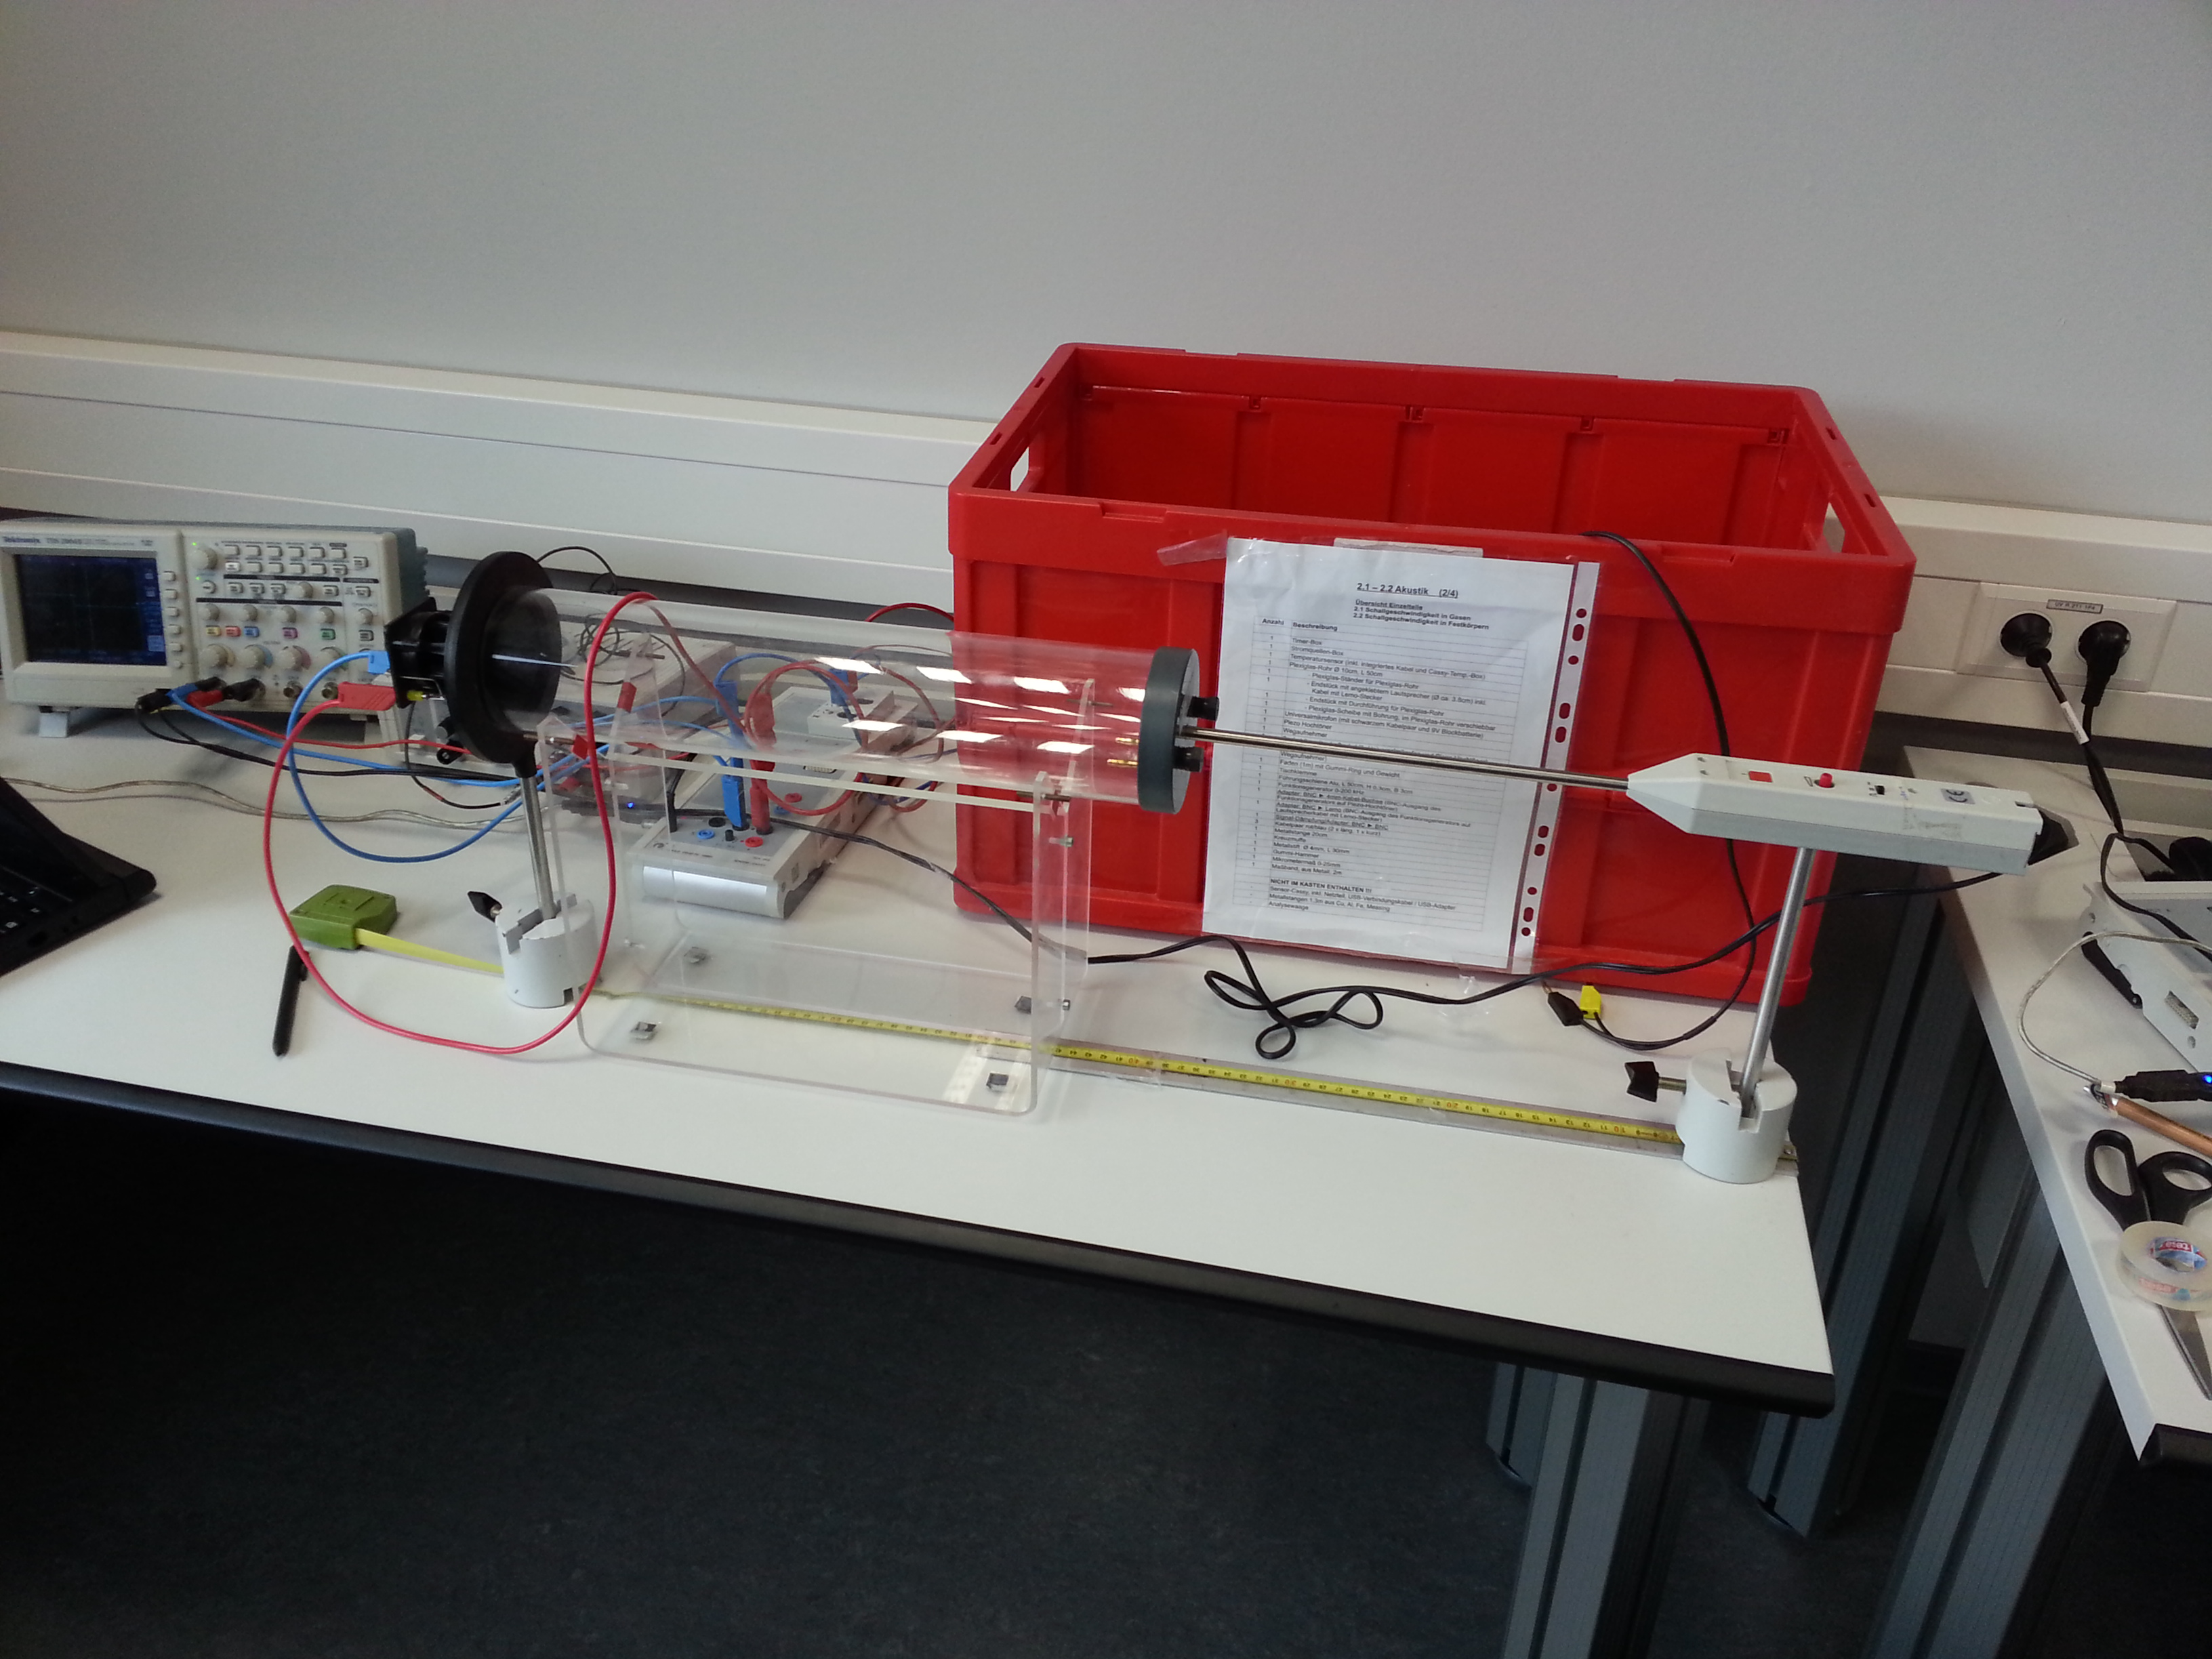
\includegraphics[scale=0.15]{Bilder/laufzeit-oszi.jpg}
\caption{Versuchsaufbau der Laufzeitmessung mit dem Oszilloskop.}
\end{figure}


Bei dem Versuch wurde mit einem Piezo-Hochtöner am einen Ende eines Schallrohrs eine Störung erzeugt, die dann in verschiedenen Abständen innerhalb des Schallrohrs von einem Mikrofon im Trigger-Modus aufgezeichnet wurde. Der Piezo-Hochtöner wurde sowohl an eine Timerbox, die an das Sensor-Cassy anschlossen wurde, als auch parallel dazu an das Relais des Sensor-Cassys angeschlossen. Das Mikrofon wurde ebenfalls an die Timerbox angeschlossen. Beim Start der Messung wird das Relais geschlossen, wodurch das Piezoelement entladen wird und die Störung aussendet. Nach Schließen des Relais wird dieses wieder aufgeladen. Beim  Eintreffen der Störung am Mikrofon, liefert dieses das Stopp-Signal für die Zeitmessung.
Anschließend wurde dieser Versuch noch einmal mit einem Oszilloskop aufgezeichnet und der Abstand der Spannungspeaks mit Hilfe des Cursors abgelesen.
Außerdem wurde während des Versuchs die Temperatur der Luft gemessen.
\newpage
\subsection{Versuchsauswertung}
\subsubsection{Rohdaten}
\begin{figure}[H]
\centering
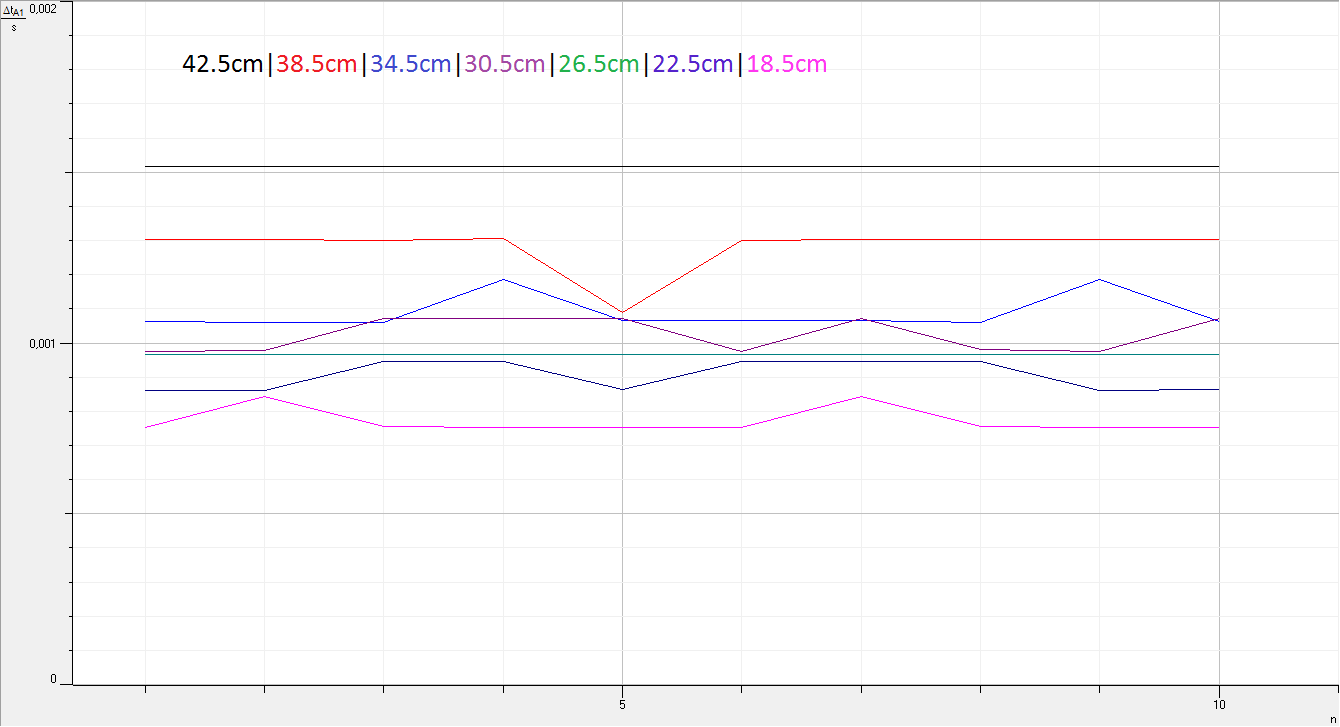
\includegraphics[scale=0.6]{Bilder/Rohdaten-Laufzeitmessung.png}
\caption{Beispiel einer Laufzeitmessung mit dem Sensor-Cassy bei verschiedenen Abständen}
\label{Laufzeitrohdaten}
\end{figure}
\begin{figure}[H]
\centering
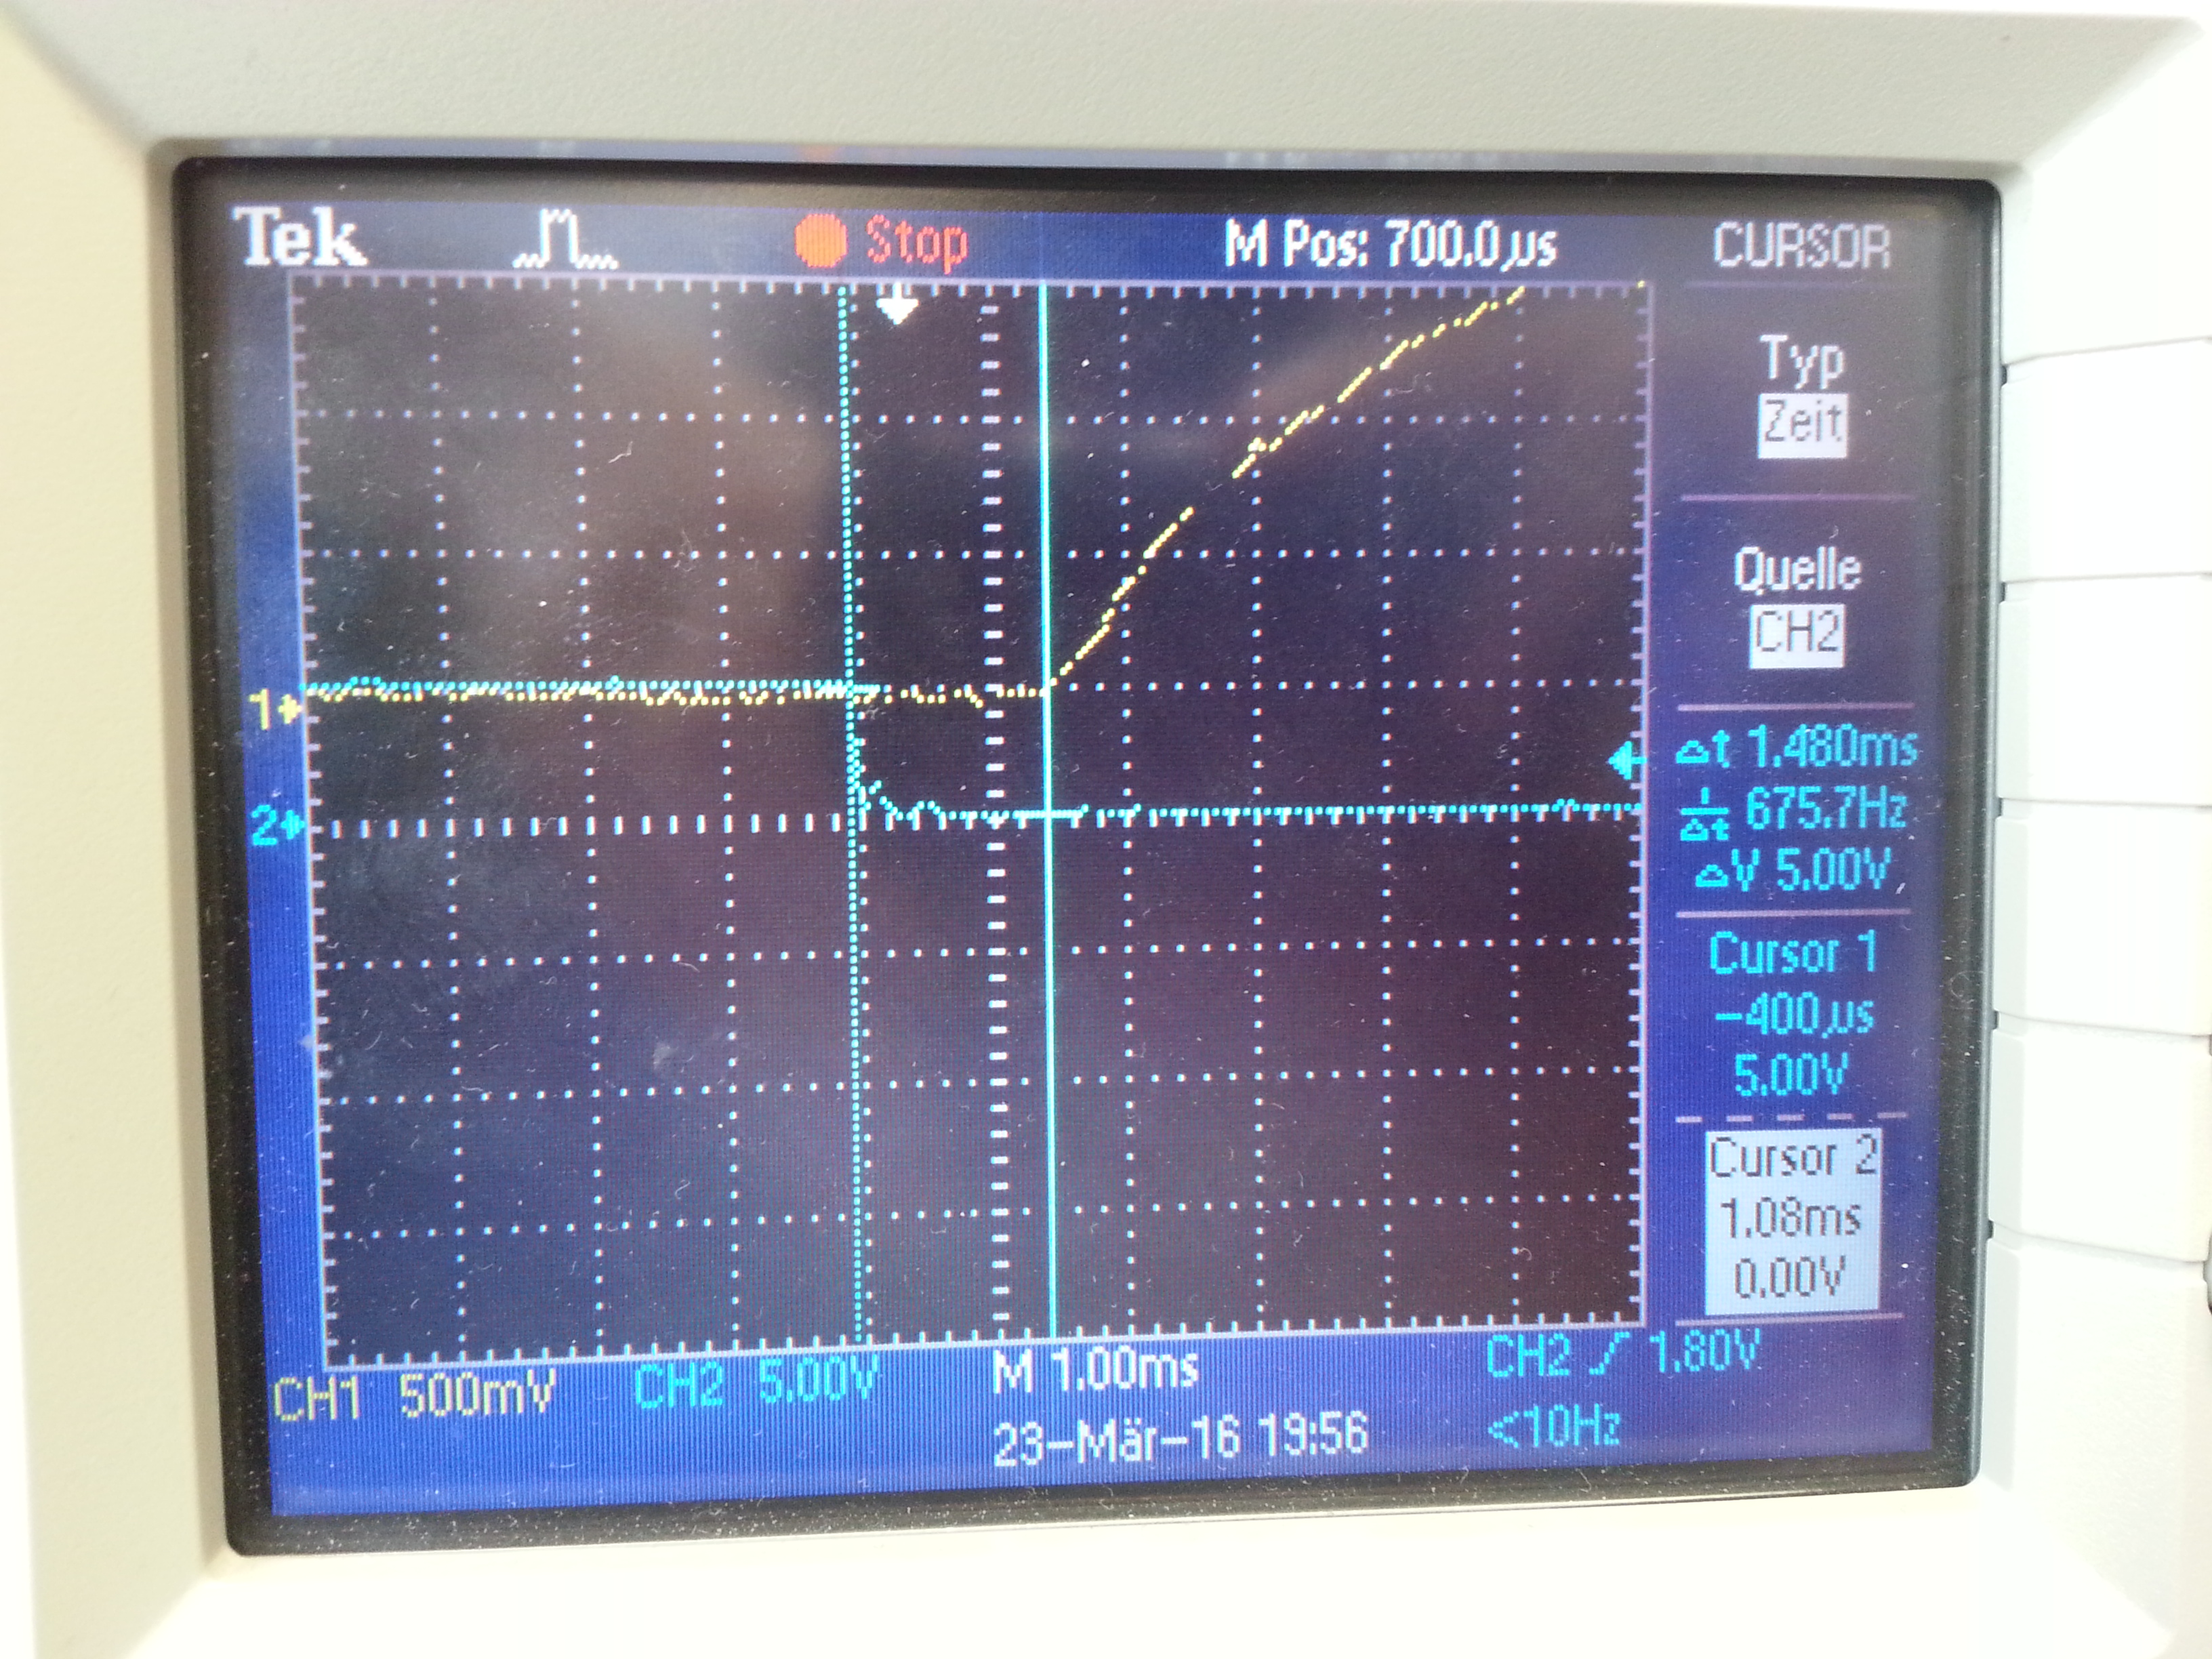
\includegraphics[scale=0.12]{Bilder/oszi.jpg}
\caption{Beispiel einer Laufzeitmessung mit dem Oszilloskop bei einem Abstand von 42.5cm}
\end{figure}
\begin{table}[H]\centering
\caption{Werte der Laufzeitmessung mit dem Oszilloskop}
\begin{tabular}{c|c}
Abstand in m & Zeitdifferenz der Spannungspeaks in ms\\ 
\hline
$42.5$& $1.48$\\ 
$34.5$& $1.24$\\
$26.5$& $1.08$\\
\end{tabular} 
\end{table}
Der Fehler auf die Zeit ergibt sich aus der Auflösung des Oszilloskops zu $0.04ms$.
Die Lufttemperatur betrug während des Versuchs ca. $22.6^{\circ}C$.
\subsubsection{Transformation der Rohdaten/Analyse}
Zur Auswertung wurden die gemessenen Werte der Cassy-Messung für die Zeit bei den jeweiligen Abständen gemittelt und die Fehler bestimmt.
\begin{table}[H]\centering
\caption{Mittelwerte der Cassy-Laufzeitmessung mit Fehlern}
\begin{tabular}{c|c|c}
Abstand in m & Mittelwert der Zeit in ms & $\sigma_t$ in ms\\ 
\hline
$42.5$& $1.51705$& $4.104 \cdot 10^{-4}$\\ 
$38.5$& $1.28692$& $7.141 \cdot 10^{-2}$\\
$34.5$& $1.08284$& $4.526 \cdot 10^{-2}$\\
$30.5$& $1.05089$& $4.390 \cdot 10^{-2}$\\
$26.5$& $0.96639$& $5.193 \cdot 10^{-4}$\\
$22.5$& $0.92490$& $3.756 \cdot 10^{-2}$\\
$18.5$& $0.80627$& $4.416 \cdot 10^{-2}$\\
\end{tabular} 
\end{table}
$~$\newline
Die Mittelwerte mit ihren Fehlern wurde anschließend gegen den Abstand des Mikrofons aufgetragen, eine Lineare Regression durchgeführt und die dazugehörigen Residuen bestimmt.
\newline
Die Auswertung der Daten des Oszilloskops erfolgte analog, nur dass wir keine Werte mitteln mussten.
\begin{figure}[H]
\centering
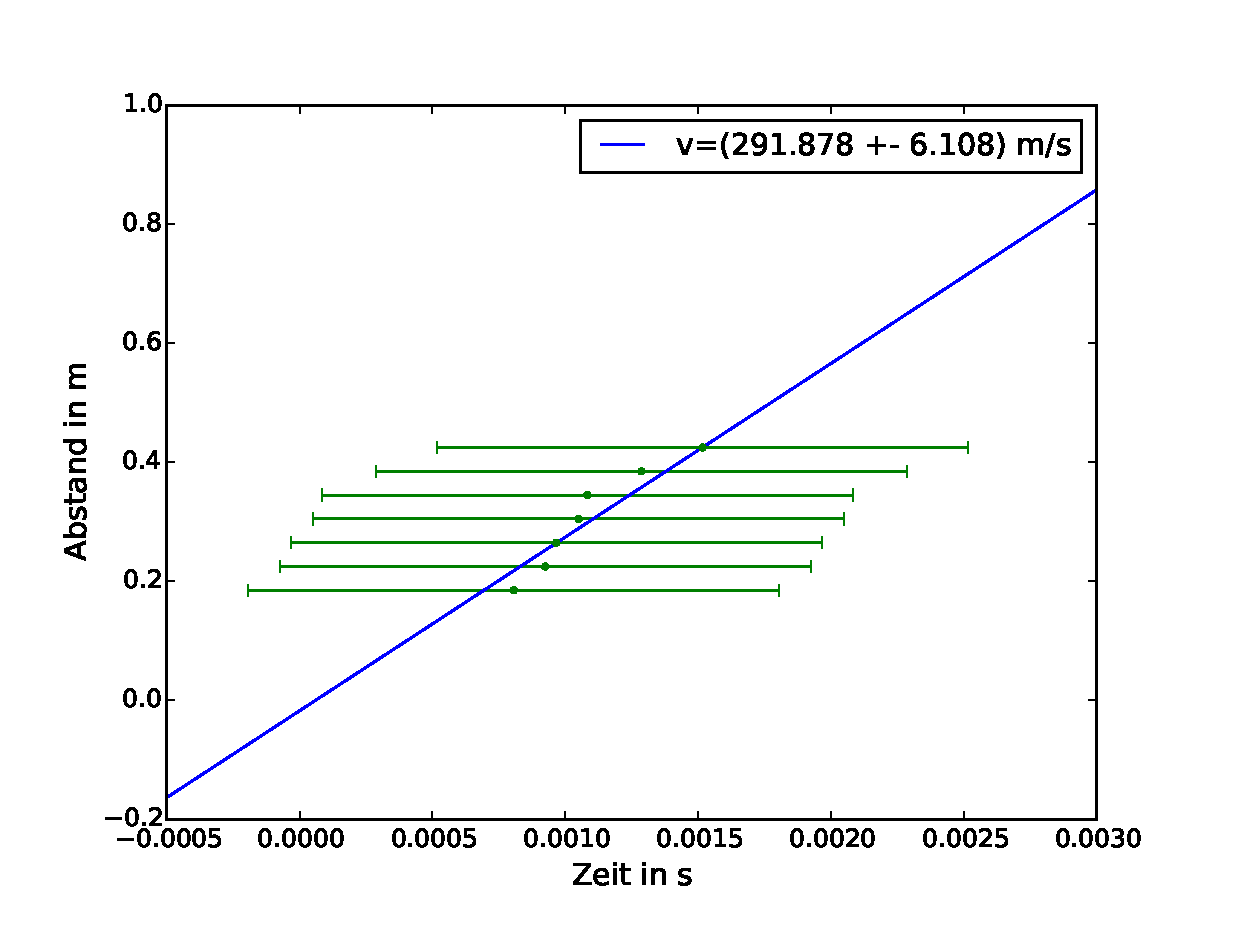
\includegraphics[scale=0.79]{Bilder/Linreg-Laufzeit.eps}
\caption{Lineare Regression durch die Mittelwerte der Cassy-Messung mit ihren Fehlern}
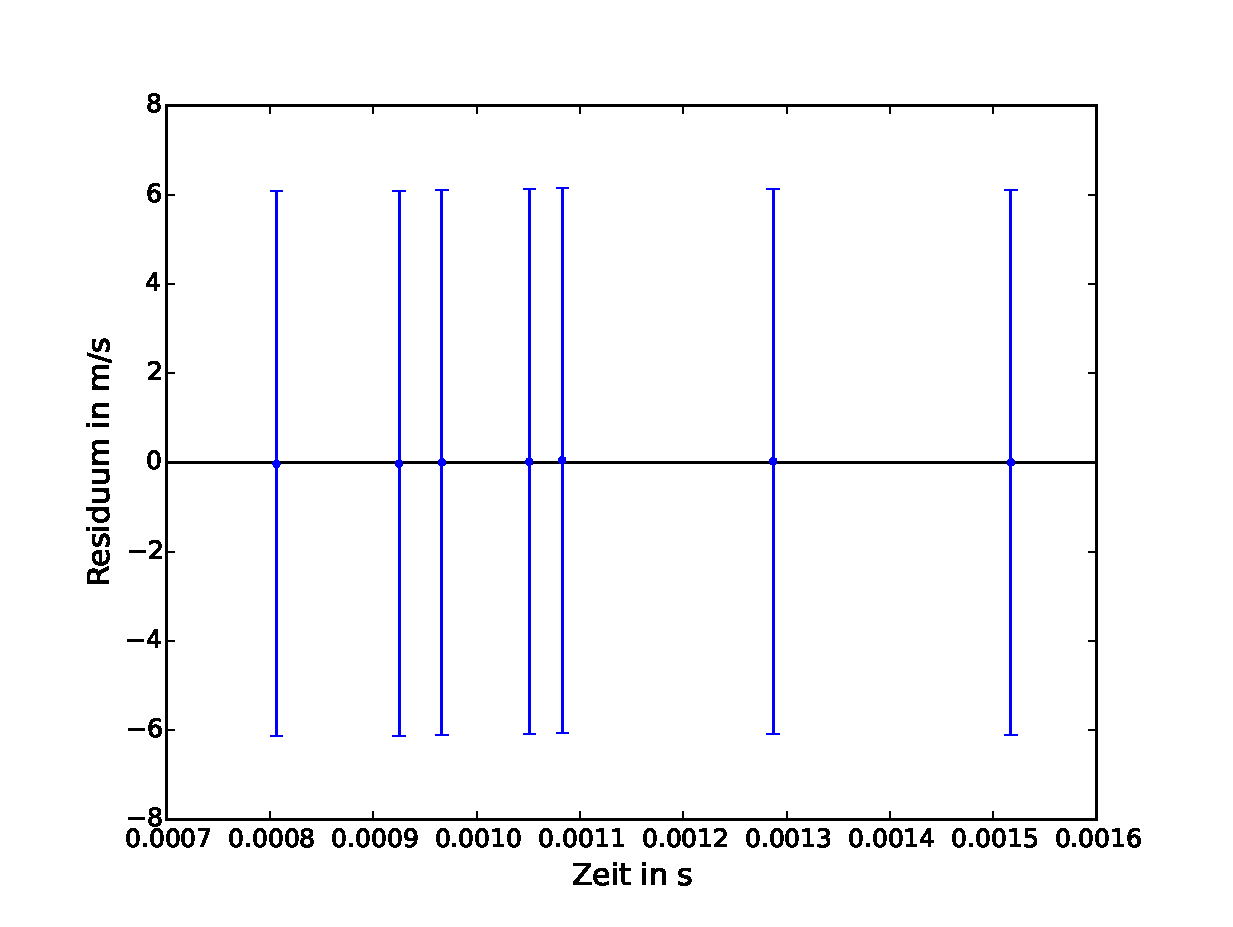
\includegraphics[scale=0.79]{Bilder/Residuen-Laufzeit.eps}
\caption{Residuen des Fits, der Cassy-Messung}
\end{figure}
\begin{figure}[H]
\centering
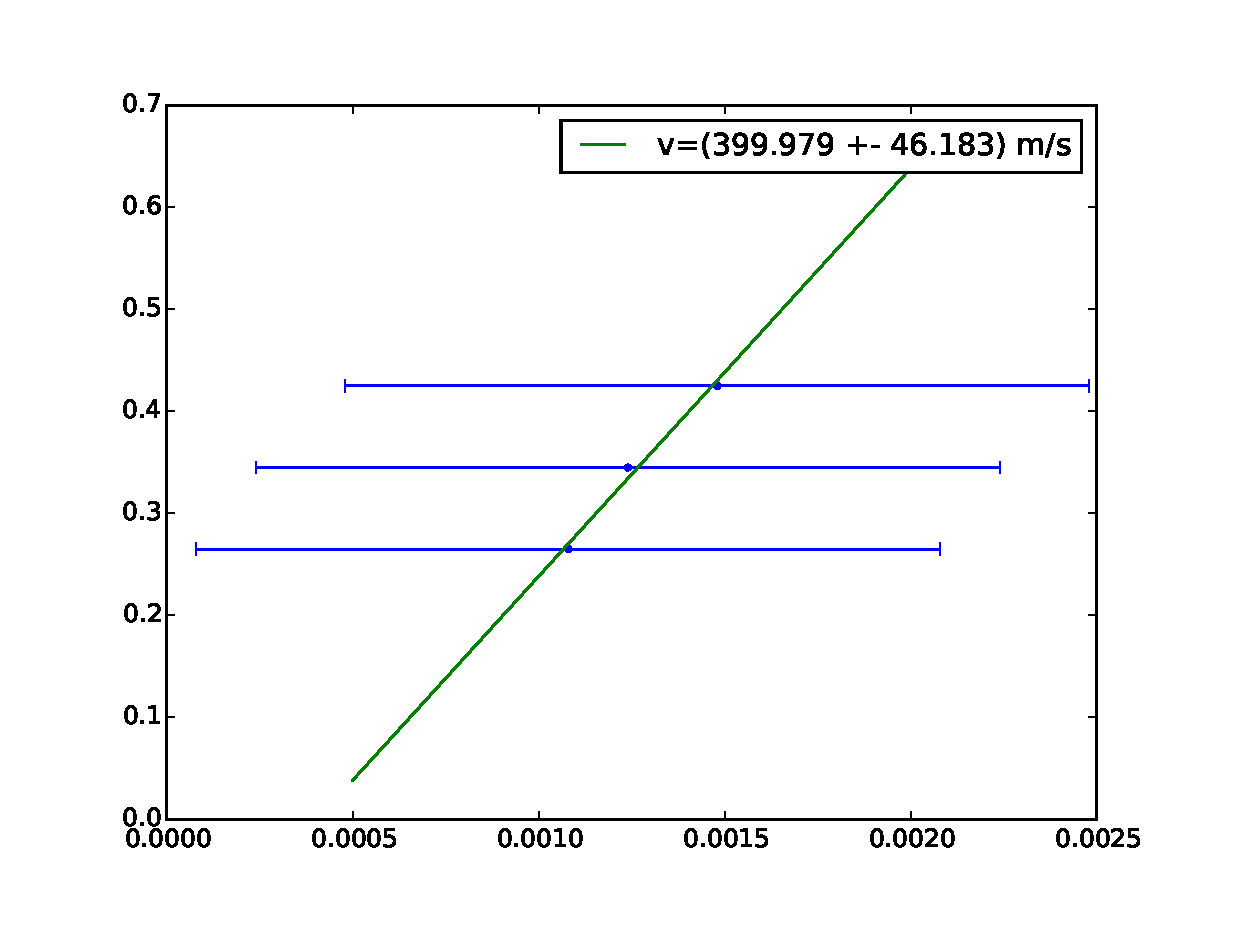
\includegraphics[scale=0.8]{Bilder/Linreg-Oszi.eps}
\caption{Lineare Regression der vom Oszilloskop abgelesenen Werte mit ihren Fehlern}
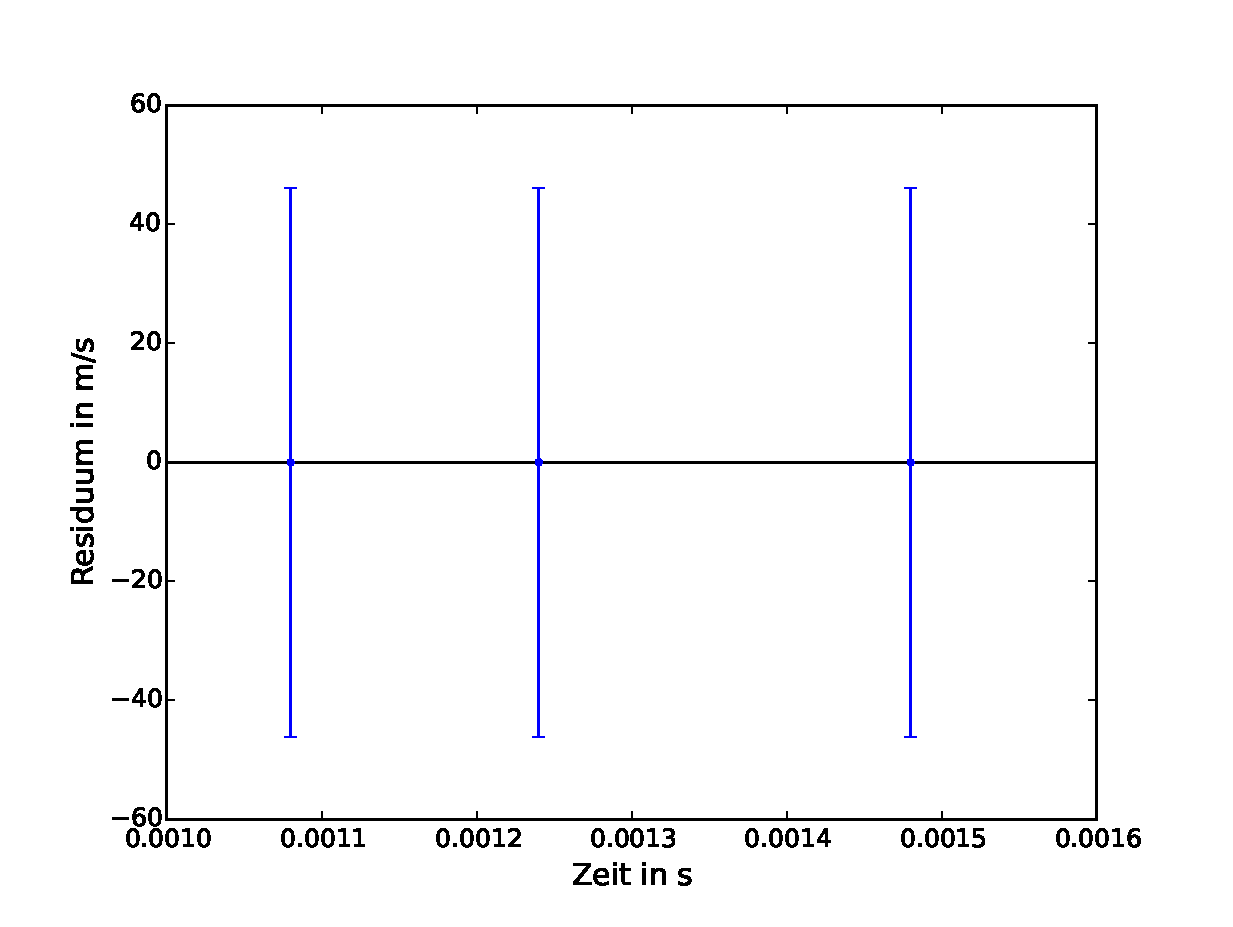
\includegraphics[scale=0.8]{Bilder/Residuen-Oszi.eps}
\caption{Residuen des Fits der Oszilloskop-Messung}
\end{figure}
$~$\newline
Als Ergebnis für die Schallgeschwindigkeit in Luft erhalten wir also einen Wert von \newline $v=(291.878 \pm 6.108) \frac{m}{s}$ für die Cassy-Messung und einen Wert von\newline $v=(399.979 \pm 46.183)\frac{m}{s}$.
\subsubsection{Fazit}
Der Literaturwert der Schallgeschwindigkeit in Luft beträgt bei einer Temperatur von $20^{\circ}C$, $342.46\, \frac{m}{s}$. Mit Gleichung (\ref{Temperaturabhängigkeit}) ergibt sich damit ein Wert von $344.98 \, \frac{m}{s}$.
Unser Ergebnis von $v=(291.878 \pm 6.108) \frac{m}{s}$ bei der Cassy-Messung weicht damit um $8\sigma$ vom Literaturwert ab. Dies erklären wir uns durch starke Streuung unserer Messwerte, bei ein und der selben Distanz (siehe Abbildung (\ref{Laufzeitrohdaten})). \newline
Unser Ergebnis von $v=(399.979 \pm 46.183)\frac{m}{s}$ bei der Oszilloskop-Messung weicht um etwas mehr als $1\sigma$ vom Literaturwert ab und ist somit völlig zufriedenstellend.

\end{document}